\newcommand{\s}[1]{
	\(\mathcal{#1}\)}

\chapter{Problema de optimizare}

Toate programele date ca exemplu sunt scrise într-un pseudo cod inspirat
din limbajul Python.

\section{Formalizarea problemei}

Fie programul \s{P} un proiect Java, format dintr-o mulțime de fișiere
clasă.  Scopul optimizatorului este să creeze un program \s{P'}, care
să se comporte identic cu \s{P}, și să fie mai bun decât
\s{P} pentru o anumită metrica \s{M}.

\section{Diferențierea programelor}

Doua programe \s{P} și \s{Q} pot fi diferențiate dacă
exista un input \s{I} pentru care \s{P} rulat pe \s{I}
și \s{Q} rulat pe \s{I} dau rezultate diferite.

\(\exists \mathcal{I}\) pentru care \(\mathcal{P}(\mathcal{I}) \ne
\mathcal{Q}(\mathcal{I}) \)

Unde prin rezultat înțelegem atât output-ul programului, în
sensul pur matematic, cât și efectele laterale generate, care au
efect asupra mediului unde rulează programul.

Dacă doua programe nu pot fi diferențiate (i.e., pentru toate
input-urile \s{I}, cele doua programe se comporta la fel), vom
spune despre ele ca sunt echivalente.

De exemplu, fie \s{P}

\begin{lstlisting}[language=Python,label={programul_p}]
def P(a: int, b: int) -> int:
    for i = 1:b
        a = inc(a)
    return a
\end{lstlisting}

Și fie \s{Q}

\begin{lstlisting}[language=Python,label={programul_q}]
def Q(a: int, b: int) -> int:
    return a + b
\end{lstlisting}

Atunci pentru orice a și b din $\N$, \s{P}(a, b) va fi egal cu
\s{Q}(a, b).

\section{Metrici de optimizare}

În contextul optimizării de programe este nevoie să definim ce
înseamnă ca dintre doua programe echivalente \s{P} și \s{Q}, \s{P}
să fie mai performant decât \s{Q}.
Cele mai folosite doua metrici sunt metrica de viteză de
execuție a unui program, și metrica de dimensiune a programului.

\subsection{Metrica de viteza}

\subsubsection{Timpul de rulare}

Vom defini timpul de rulare al unui program \s{P} pe un input
\s{I} ca fiind diferența de timp dintre când programul își începe
execuția, până când acesta își termină execuția.

Pe sistemele *nix, un mod ușor a măsura timpul de rulare este
folosind comanda $time$:

\begin{lstlisting}[language=Bash]
$ time ./build.sh
./build.sh  0.47s user 0.20s system 100% cpu 0.664 total
\end{lstlisting}

În acest context, vom spune ca programul $build.sh$ a rulat
pentru un timp de 0.664 secunde.

Vom defini astfel \[time(\mathcal{P}, \mathcal{I})\] ca fiind
timpul de rulare al programului \s{P} pe input-ul \s{I}.

\subsubsection{Comparare bazata pe timpul de rulare}

Fie doua programe echivalente \s{P} și \s{Q}.

Vom spune că \s{P} este mai rapid decât \s{Q} pe baza timpului de
rulare dacă timpul de rulare mediu al lui \s{P} este mai mic
decât timpul de rulare mediu al lui \s{Q}:

\[
	\sum_{\mathcal{I} \ input} time(\mathcal{P}, \mathcal{I}) <
	\sum_{\mathcal{I} \ input} time(\mathcal{Q}, \mathcal{I})
\]

Pe baza acestei comparații, putem defini o relație de ordine
asupra mulțimii programelor: \s{P} $\textless$ \s{Q} dacă \s{P}
este mai rapid decât \s{Q}.

\subsubsection{Problema optimizării pe baza metricii de viteza}

Având definită relația de ordine, problema optimizării pe
baza metricii de viteza este:

Dându-se un program \s{P}, să se găsească \s{Q} ca cel mai rapid
program echivalent cu \s{P}.

\subsection{Metrica de dimensiune}

\subsubsection{Dimensiunea unui program}

Pentru un program \s{P}, vom defini dimensiunea acestuia ca fiind
suma dimensiunilor tuturor instrucțiunilor acestui program:

\[
	size(\mathcal{P}) = \sum_{i\ \in\ \mathcal{P}} instruction\_size(i)
\]

Unde prin \( instruction\_size(i) \) înțelegem numărul de octeți
ocupați de instrucțiunea $i$.

De exemplu, pentru limbajul Java, instrucțiunea $invokedynamic$
ocupă 5 octeți, în timp ce instrucțiunea $dmul$ ocupă un singur
octet.

\subsubsection{Comparare bazată pe dimensiunea programelor}

Pentru doua programe \s{P} și \s{Q}, vom spune ca \s{P} este mai
mic decât \s{Q} dacă \(size(\mathcal{P}) < size(\mathcal{Q})\).

Similar ca la metrica de viteza, putem defini o relație de ordine
pe mulțimea programelor.

\subsubsection{Problema optimizării pe baza metricii de
	dimensiune}

Având definită relația de ordine, problema optimizării pe
baza metricii de dimensiune este aceeași ca la metrica de viteză:

Dându-se un program \s{P}, să se găsească \s{Q} cel mai mic
program echivalent cu \s{P}:

\[
	\operatorname*{argmin}_\mathcal{Q} \mathcal{P}
	\text{ echivalent cu  } \mathcal{Q}
\]

\section{Discuție asupra metricilor}

Pentru cele mai multe cazuri, cele doua metrici sunt corelate --
o reducere a dimensiunii programului aduce cu ea și o reducere a timpului de rulare.

Totodată, exista cazuri când cele doua metrici sunt contrare.
Un exemplu clasic este tehnica de "derularea buclelor" (Eng. "Loop
unrolling").
Aceasta constă în explicitarea unei bucle cu un număr cunoscut
de iterații:

Programul
\begin{lstlisting}[language=Python]
s = 0
for i = 1:10:
    s = inc(s)
\end{lstlisting}

Va fi optimizat pentru viteză în
\begin{lstlisting}[language=Python]
s = 0
s = inc(s))
...
s = inc(s))
\end{lstlisting}

În timp ce această optimizare va crește numărul de instrucțiuni
al programului, deci și dimensiunea acestuia.

Deoarece cele mai multe programe utilizate nu rulează pe medii
constrânse de memorie, tipul de optimizare folosit aproape
întotdeauna este cel de viteza: este mult mai util dacă un
program rulează de 2 ori mai repede, decât dacă acesta ocupă de
2 ori mai puțin spațiu.

Acest lucru se datorează faptului că performanța memoriei (prețul
per unitate de memorie) a continuat să scadă în ultimul deceniu,
în timp ce performanța procesoarelor (numărul de instrucțiuni
executate per secundă) a stagnat.

Asa cum se poate observa în figura \ref{fig:cpu_and_gpu_trends},
trendul care urma legea lui Moore \cite{moores_law} a început să
se oprească. Pe de altă parte, eficiența memoriei calculatoarelor
și-a continuat trendul de creștere, așa cum se poate observa în figura
\ref{fig:memory_trends}.

\begin{figure}
	\centering
	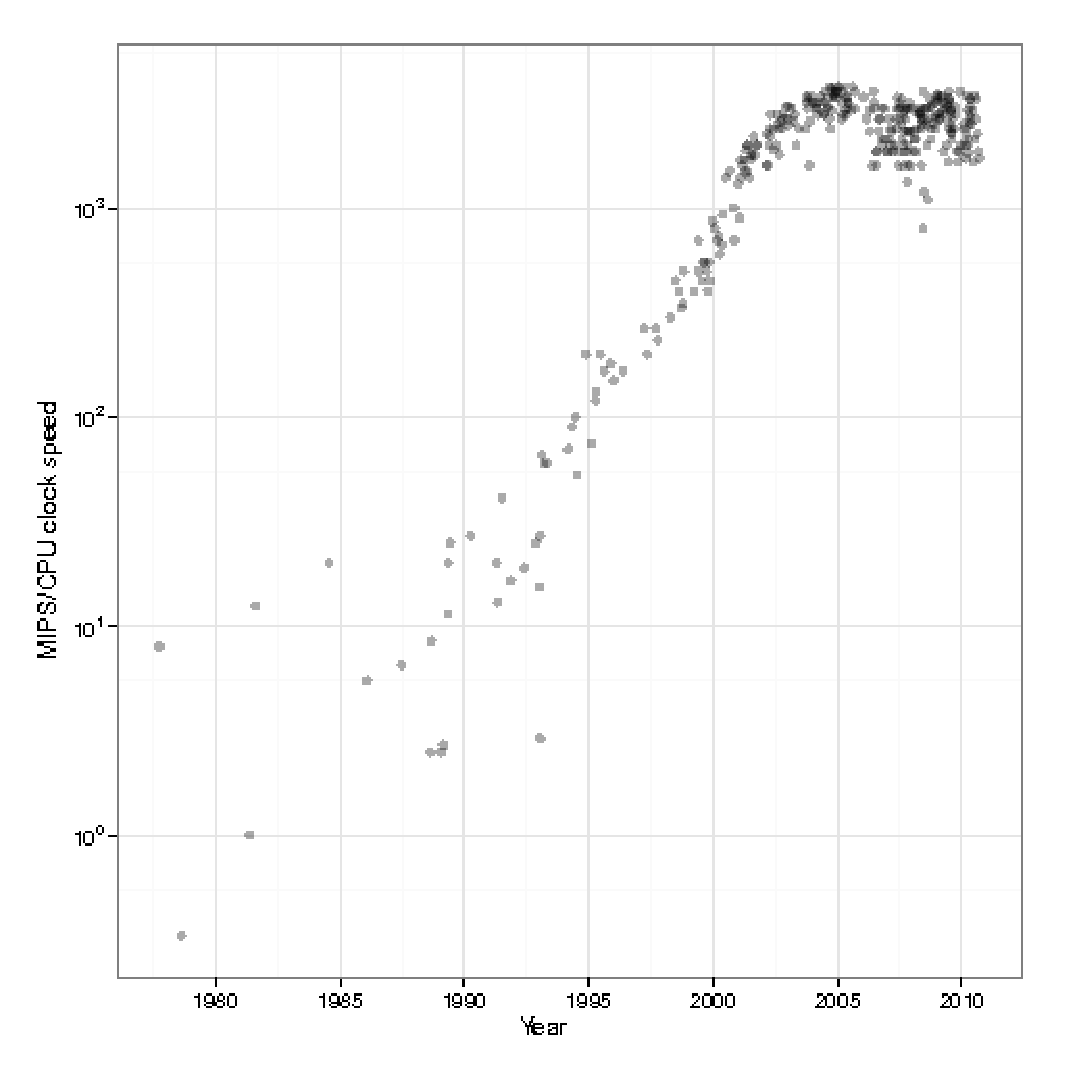
\includegraphics[width=0.5\textwidth]{cpu_and_gpu_trends}
	\caption{Evoluția puterii de procesare\cite{cpu_and_gpu_trends} }
	\label{fig:cpu_and_gpu_trends}
\end{figure}

\begin{figure}
	\centering
	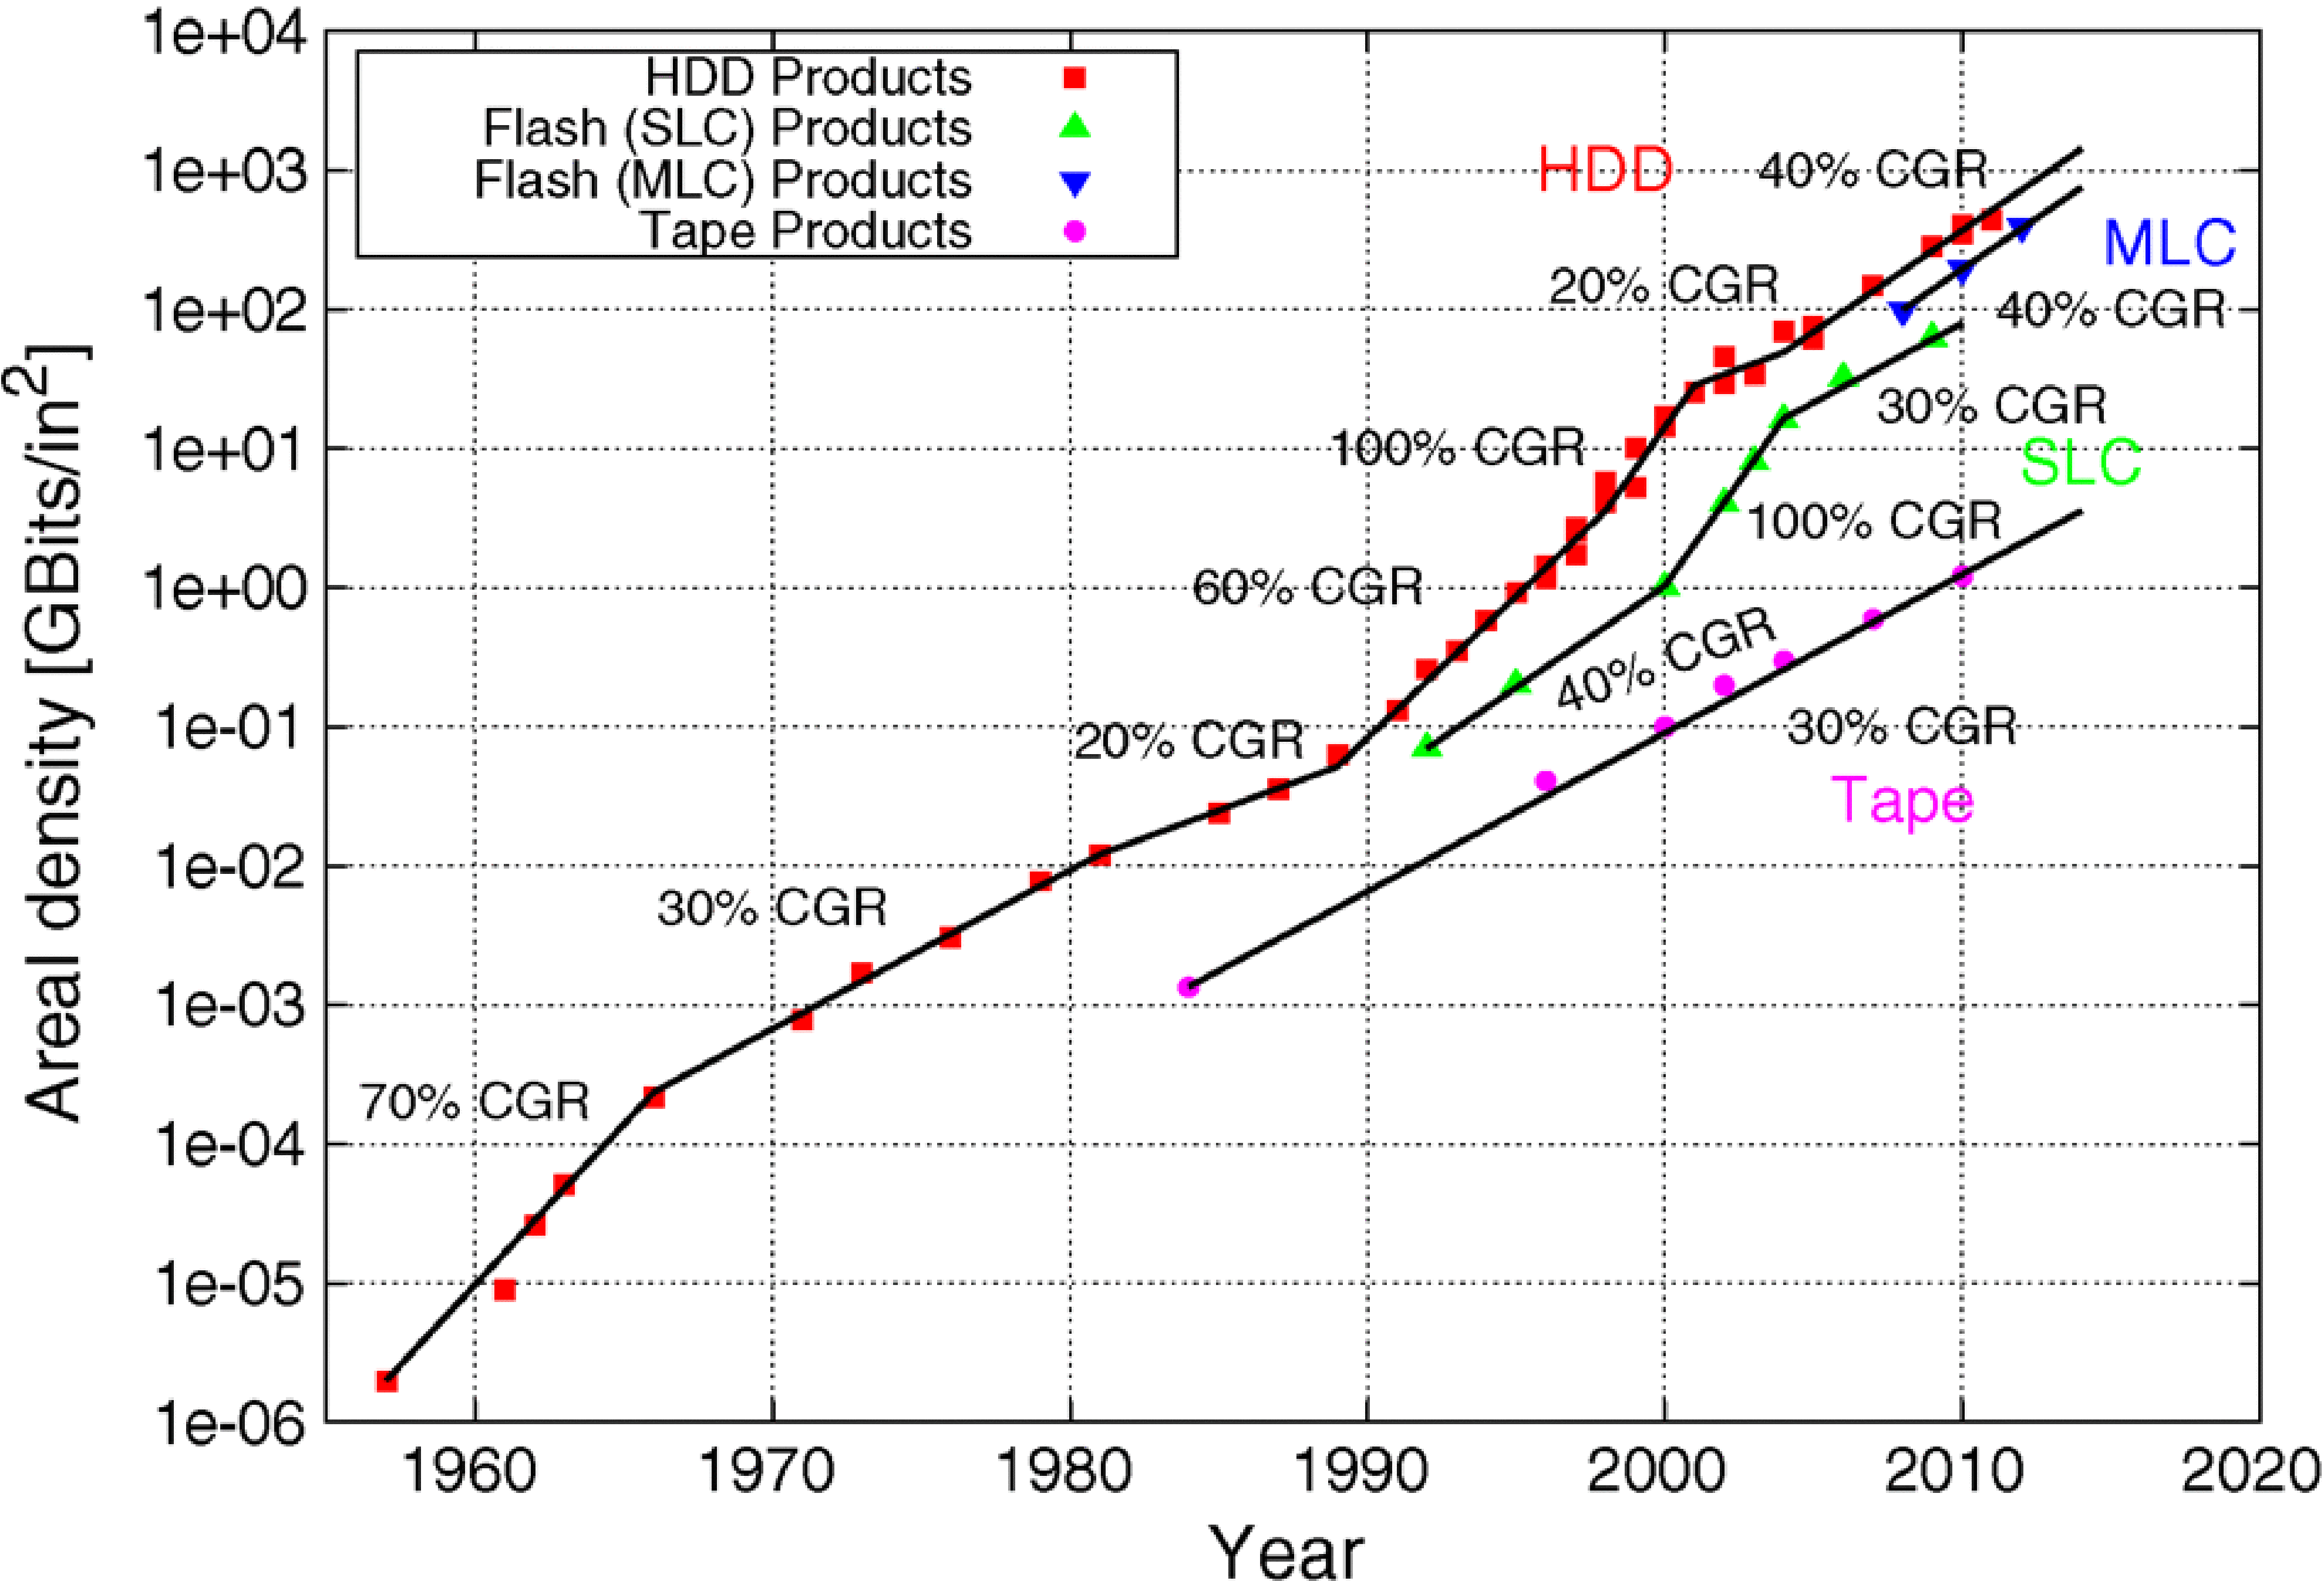
\includegraphics[width=0.5\textwidth]{memory_trends}
	\caption{Evoluția puterii de procesare\cite{memory_trends} }
	\label{fig:memory_trends}
\end{figure}
